\documentclass[a4paper,12pt]{article}
\usepackage[utf8]{inputenc}
\usepackage[cm,empty]{fullpage}
\usepackage[T2A]{fontenc}
\usepackage[english, russian]{babel}
\usepackage{amssymb,amsmath,amsxtra,amsthm}
\usepackage{proof}
\usepackage[pdftex]{graphicx}
\usepackage{wrapfig}

\usepackage[left=2cm,right=2cm,
    top=1cm,bottom=1cm,bindingoffset=0cm]{geometry}

\renewcommand{\leq}{\leqslant}
\renewcommand{\geq}{\geqslant}


\newcommand{\iiff}{\Longleftrightarrow}
\renewcommand{\iff}{\Leftrightarrow}
\newcommand{\nothing}{\varnothing}

\newtheorem*{rem}{Замечание}

\newcommand{\NN}{\mathbb{N}}
\newcommand{\ZZ}{\mathbb{Z}}
\newcommand{\Q}{\mathbb{Q}}
\newcommand{\A}{\mathbb{A}}
\newcommand{\R}{\mathbb{R}}
\renewcommand{\C}{\mathbb{C}}

\renewcommand{\phi}{\varphi}
\newcommand{\eps}{\varepsilon}

\newcounter{z}


\newcommand{\zs}{\refstepcounter{z}\vskip 10pt\par\noindent
\fbox{\textbf{12.\arabic{z}}} }

\newcommand{\z}{\refstepcounter{z}\vskip 20pt\noindent
\fbox{\textbf{\arabic{z}}} }

\renewcommand{\date}{{\bf 3 февраля 2021}} %Дата занятия

\newcommand{\dif}
{
------------------------------------------------------------------------------------------------------------------------------------------------------
}

\newcommand{\HSEhat}{
\vspace*{-0pt}
\noindent
\setcounter{z}{0}
\vspace*{-10pt}
\begin{wrapfigure}[2]{l}{5pt}
\vspace*{-25pt}
\hspace*{-20pt}

\includegraphics[scale=0.18]{img/HSE_LOGO.png}
\end{wrapfigure}
\vspace{-20pt}


{\bf \phantom{\date}  \large \hfill Дискретная математика: \hfill \normalsize \date}

\vspace{5 pt}
{\bf \large \hfill  ориентированные графы и алгоритмы на графах.\hfill }

\vspace{15 pt}
\centerline{ \large  Домашнее задание.}



\vspace*{10pt}
\setcounter{z}{0}

}

\begin{document}

\HSEhat



\centerline{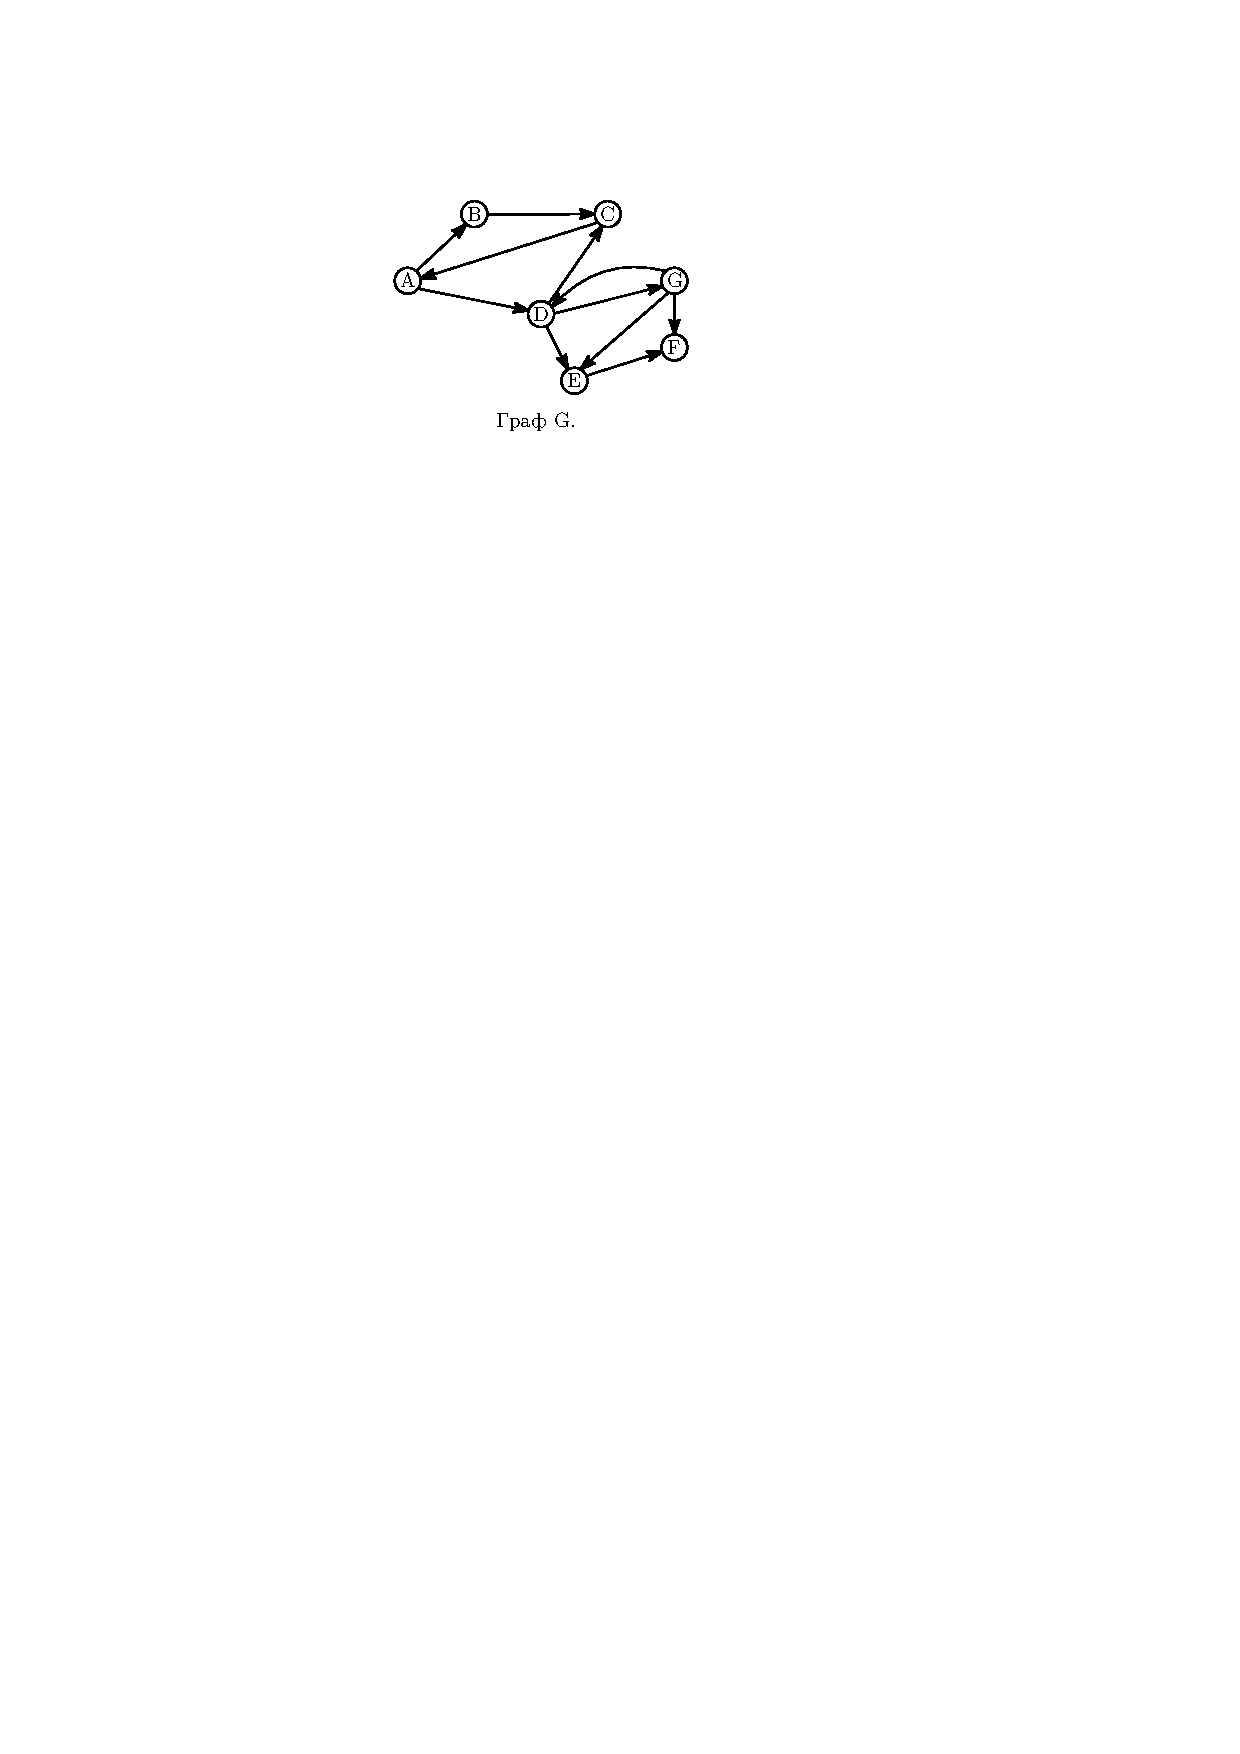
\includegraphics[scale=1.1]{img/digraphHW.pdf}\qquad \qquad 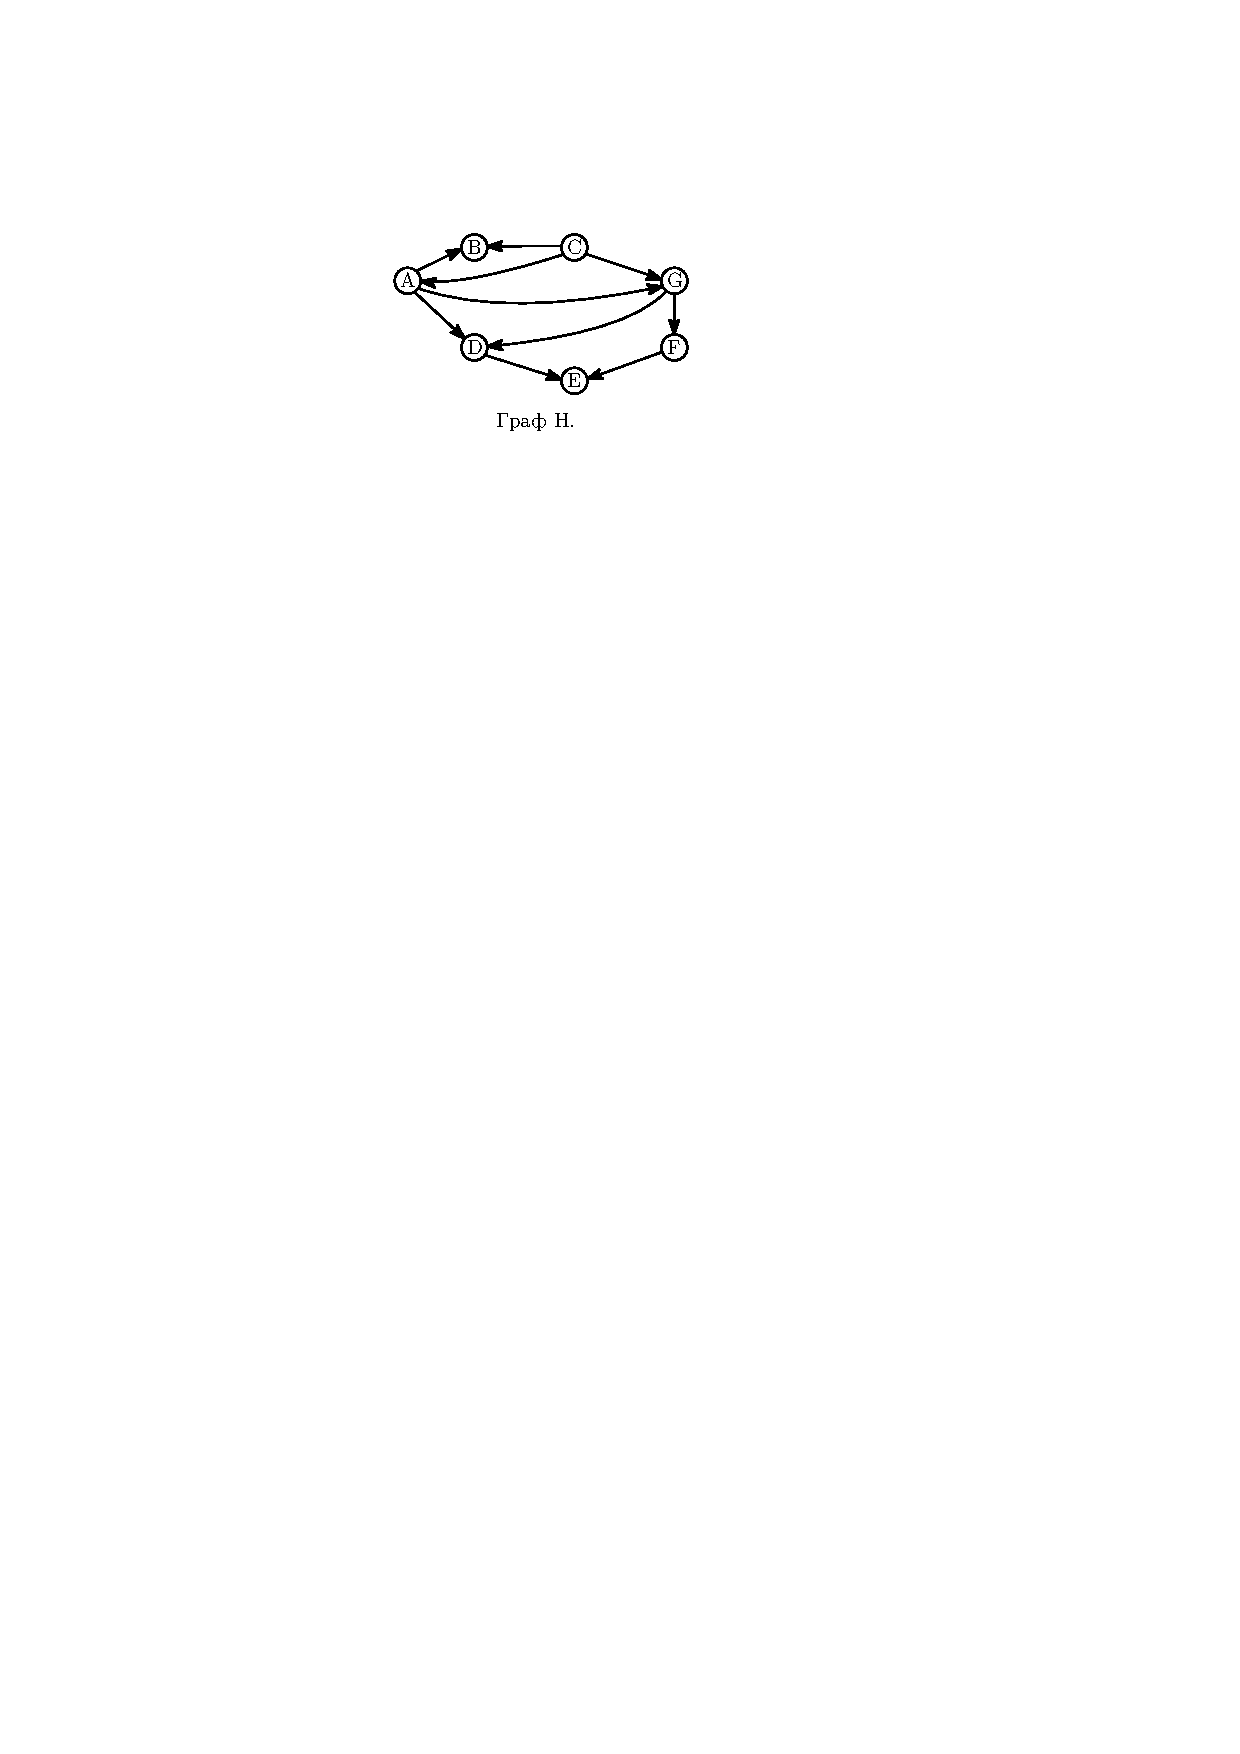
\includegraphics[scale=1.1]{img/digraphHW2.pdf}}

\z Граф $G$ изображен на рисунке выше.\\
{\bf a)} Найдите максимальную длину простого цикла в графе $G$. Укажите
все различные простые циклы максимальной длины. (Достаточно предъявить ответ)\\
{\bf б)} Найдите компоненты сильной связности графа $G$. (Достаточно предъявить ответ)\\
{\bf в)} Какое минимальное число рёбер необходимо добавить в граф $G$, чтобы
он стал сильно связным? (Необходимо обоснование ответа)

%\centerline{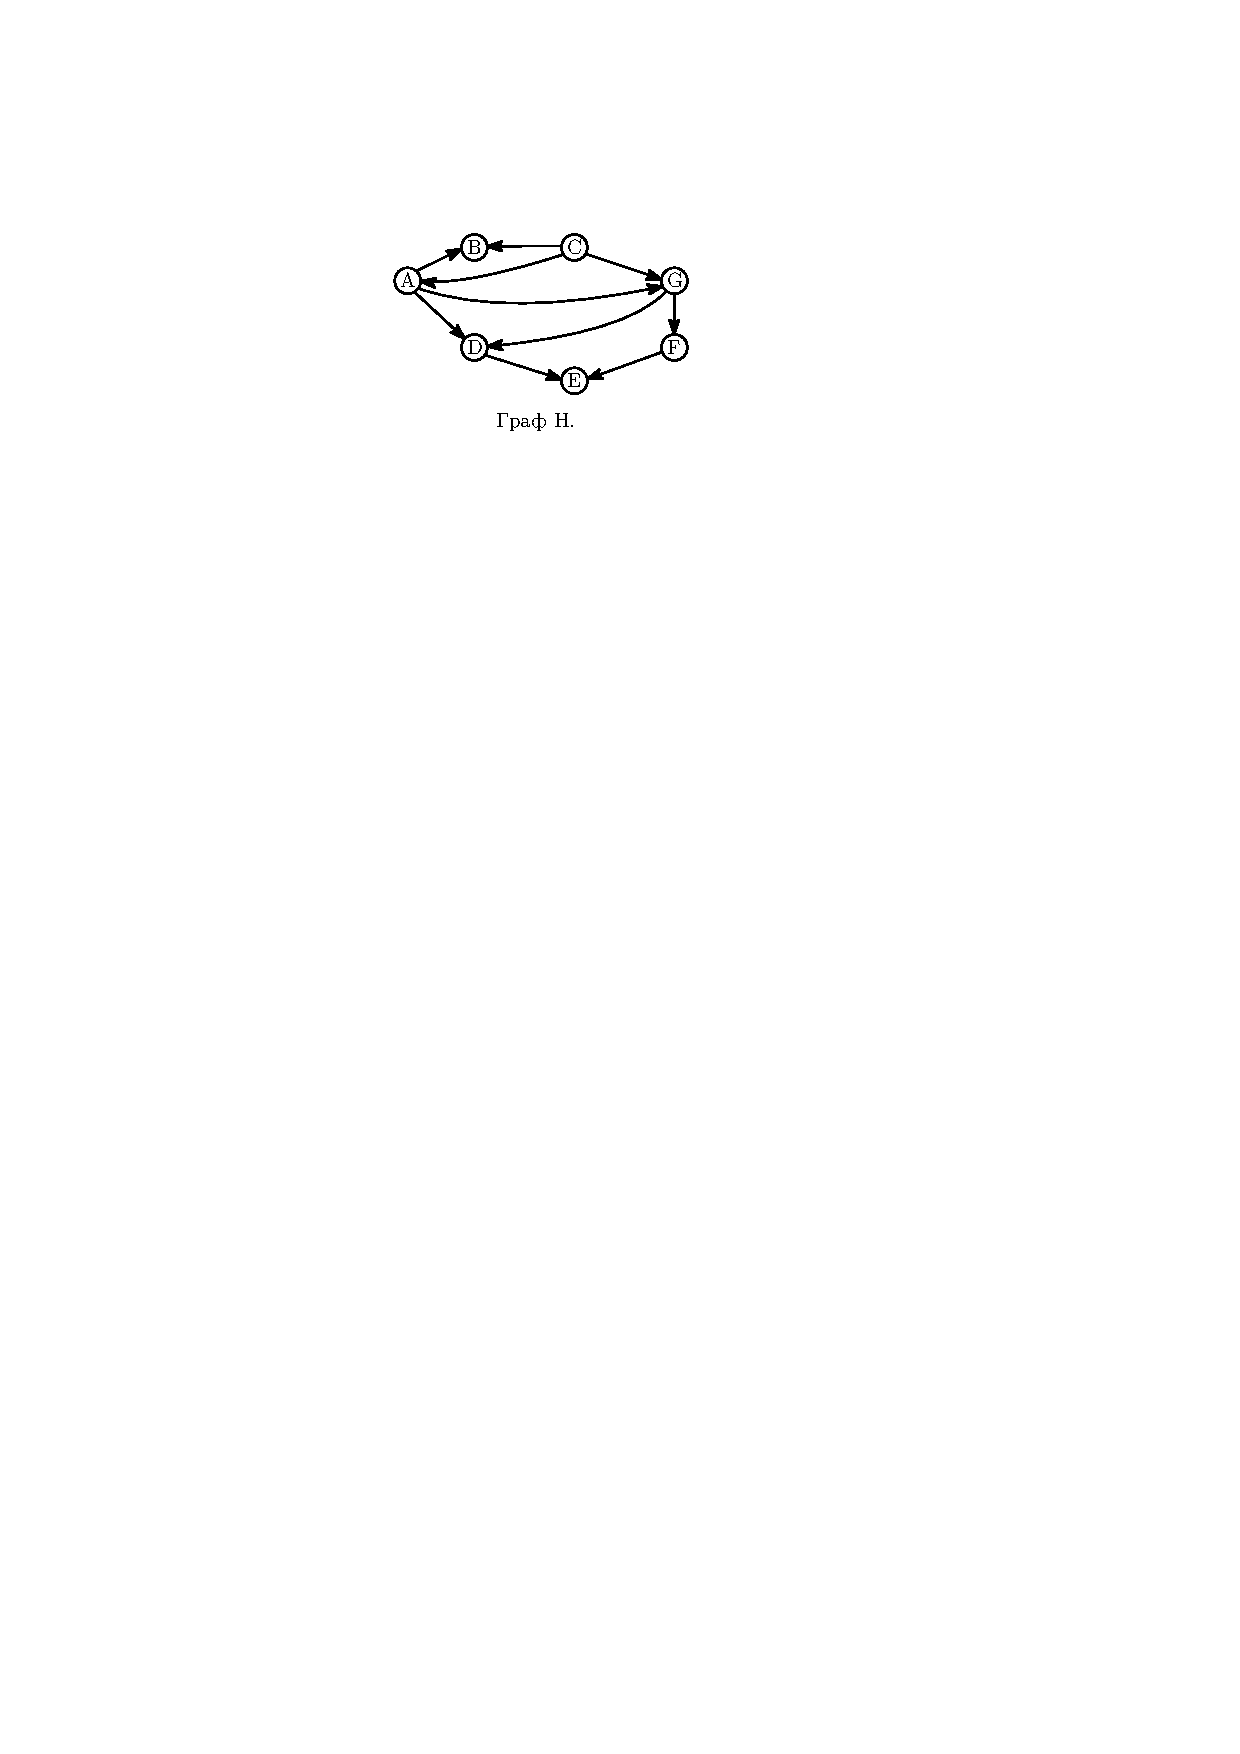
\includegraphics[scale=0.8]{img/digraphHW2.pdf}}я
\z Ациклический граф $H$ изображен на рисунке выше. Осуществите топологическую сортировку вершин графа $H$.
(Достаточно предъявить ответ. В ответе можно, например, указать последовательность вершин от меньшего номера к большему.)
\vskip 10 pt

{\it К остальным задачам необходимо привести решения с обоснованием.}

\vskip 10 pt
\centerline{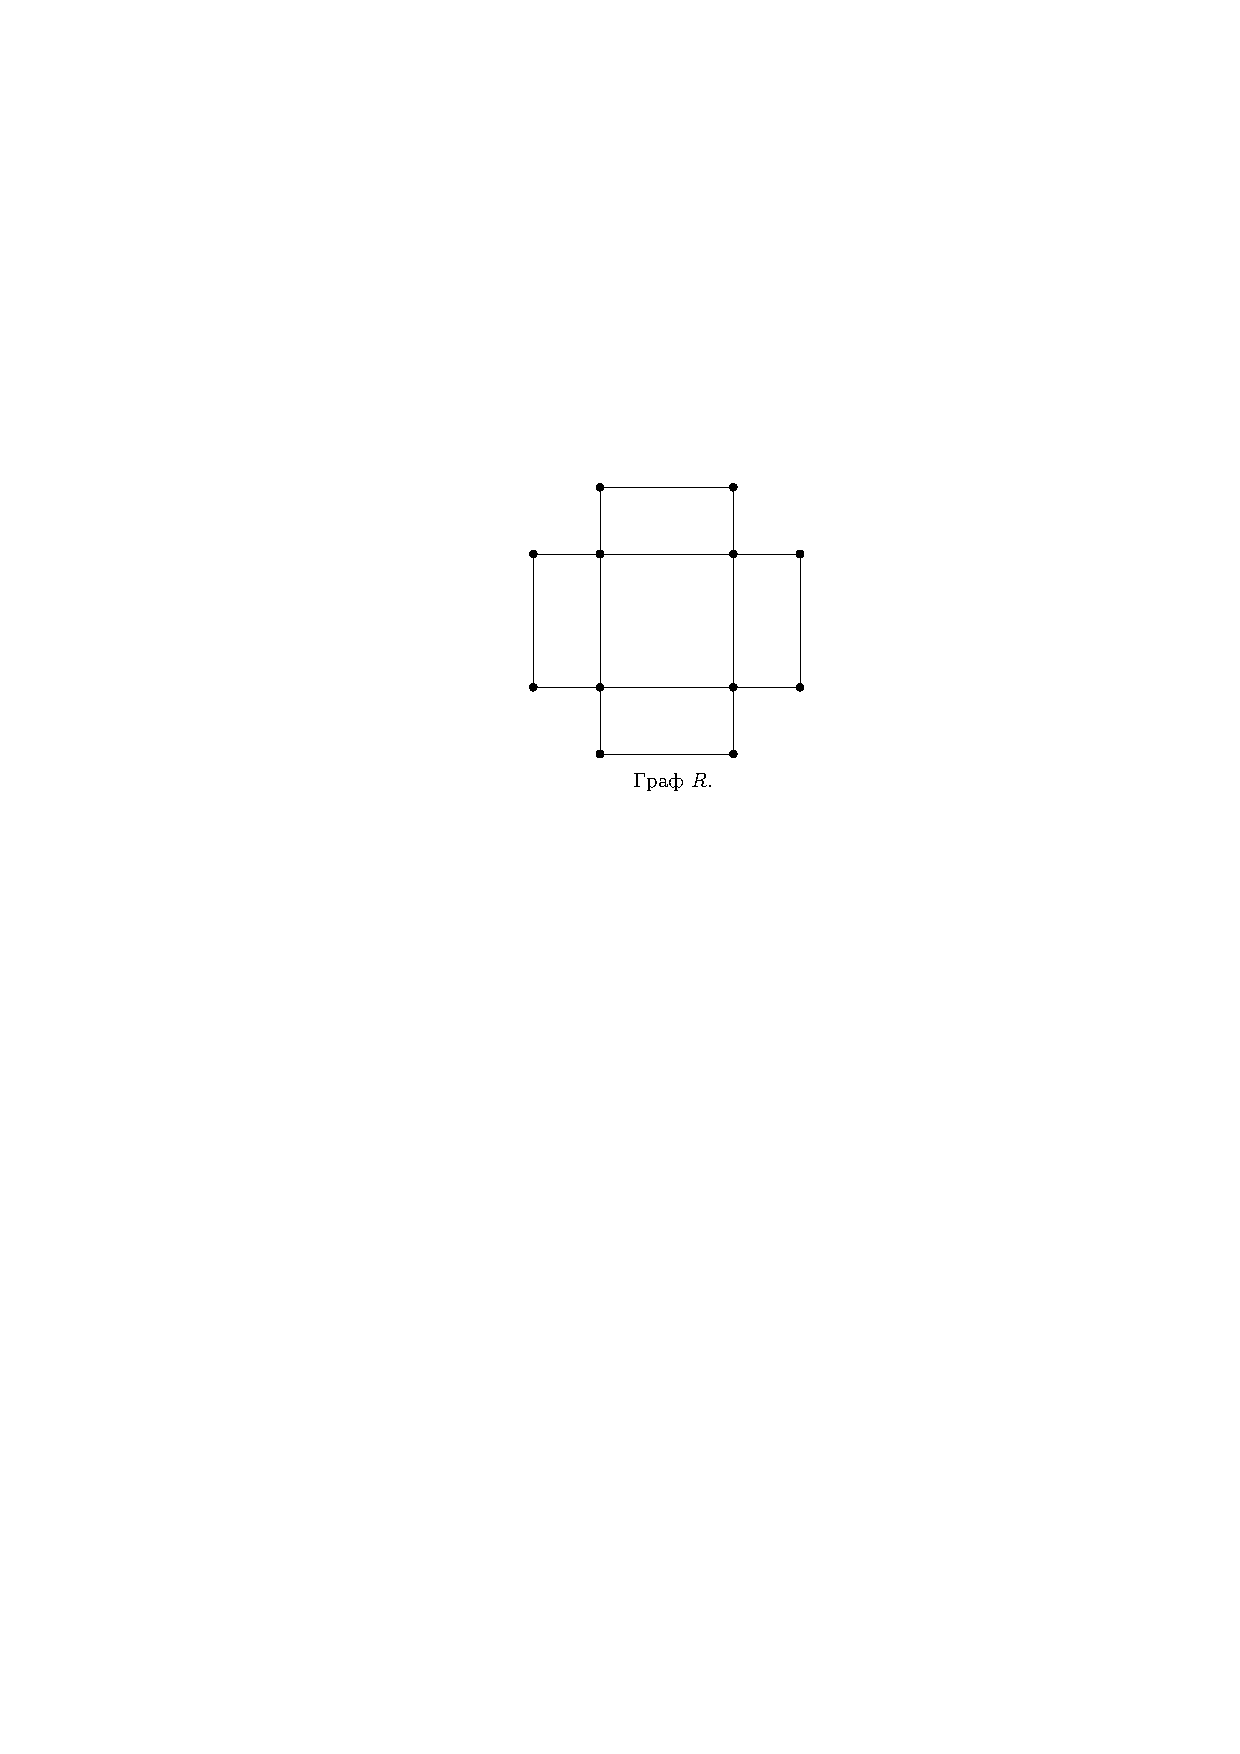
\includegraphics[scale=1.1]{img/HgraphHW.pdf}}

\z Граф $R$ изображен на рисунке выше. Верно ли, что граф $L(R)$ гамильтонов?

\z На плоскости отмечено $15$ точек, которые соединены $25$ непересекающимися отрезками так, что от любой точки можно добраться до любой другой по 
этим отрезкам.\\
{\bf а)} На сколько частей разбита плоскость этой фигурой?\\
{\bf б)} А на сколько частей разобьют плоскость $5$ таких непересекающихся фигур?

\newpage

\noindent {\bf Определение.} Напомним, что {\it правильной раскраской} графа называется такое сопоставление каждой его вершине цвета, что любым двум смежным вершинам соответствуют разные цвета.

Кроме того, на занятии было доказано, что для правильной раскраски полного графа на $n$ вершинах $K_n$ необходимо $n$ цветов.

\z В некоторой компании $7$ рабочих групп $a,b,c,d,e,f$ и $g$. В пятницу необходимо провести собрания в каждой рабочей группе по отдельности, причем каждое собрание можно планировать в один из $4$ временных слотов: \\
\centerline{9:00 - 10:45,\qquad 11:00 - 12:45,\qquad 13:15 - 15:00\quad и\quad  15:15 - 17:00.}

\noindent Кроме того, некоторые сотрудники участвуют сразу в нескольких группах:
\begin{itemize}
\item есть те, кто одновременно состоят в $a,b,c$ и $d$;

\item несколько сотрудников состоят в $g,f$ и $d$ одновременно;

\item часть состоит в группах $b,d$ и $e$ одновременно;

\item и еще один человек работает в $e$ и $f$.
\end{itemize}

Собрания в разных группах можно проводить в одно и то же время, если нет сотрудников, которые в этот момент должны быть сразу на нескольких разных собраниях.

Получится ли провести все собрания в пятницу? Какое минимальное количество временных слотов необходимо?


\z Напомним, что граф называется двудольным, если его можно правильно раскрасить в два цвета.\\
{\bf а)}  Какое наибольшее число ребер может быть в простом двудольном графе на $k$ белых и $m$ чёрных вершинах? (В нем не должно быть ребер, соединяющих вершины одинакового цвета.)\\
{\bf б)} Какое наибольшее количество рёбер может быть в двудольном графе на $2n$ вершинах?

\z Рассмотрим алфавит, состоящий только из двух букв $a$ и $b$. Все возможные слова, которые можно получить в этом алфавите, назовем языком.\\
{\bf a)} Докажите, что в этом языке можно составить слово, в котором любая трехбуквенная комбинация этих двух букв ($aaa$, $aab$, \ldots, $bba$, $bbb$) встречается ровно один раз.\\
{\bf б)} Существует ли слово, которое удовлетворяет условию предыдущего пункта и начинается на $abba$? Если существует, то укажите его. Если не существует, то объясните, почему это невозможно.

\begin{rem}
Трехбуквенная комбинация --- три подрядыдущие буквы в слове. 
\\В слове $aaaa$, например, комбинация букв $aaa$ встречается два раза (первые три буквы и последние).
А вот в слове $ababa$ три комбинации: $aba$, $bab$ и $aba$.
\end{rem}

\end{document}